\documentclass[12pt,a4paper]{article}

\usepackage[utf8]{inputenc}

\usepackage[width=190mm,height=272mm,centering]{geometry}

% \usepackage{mathptmx}
\usepackage{palatino}

%\usepackage{chancery}
%\usepackage{antiqua}
%\usepackage{aboensis}
\usepackage{gfsartemisia-euler}
\usepackage[T1]{fontenc}

% \usepackage{fontspec}
% \setmainfont{QTChanceryType}

\usepackage{graphicx}
\usepackage[table]{xcolor}
\usepackage{tikz}
\usetikzlibrary{decorations.text}
\usepackage[hidelinks]{hyperref}

\pagestyle{empty}

\newcommand{\logo}{\makebox[56mm][c]{\rule{0mm}{66mm}\raisebox{12mm}{
\includegraphics[width=48mm]{logo/aldc-4couleurs-3.pdf}}}}

%\pagecolor{yellow!5}

\usepackage{fontspec}


\begin{document}
\sffamily
\bfseries
%\color{yellow!20}
\parindent=0mm

%%%%%%%%%%%%%% FOND ET LOGOS

\unitlength=1mm
\begin{picture}(0,0)
%\put(-22,-150){\includegraphics[width=212mm]{images/lambris-chene-clair.png}}
%\put(-16,-200){\includegraphics[width=212mm]{images/lambris-chene-clair.png}}
\put(-11,-280){\includegraphics[width=212mm]{images/Fond-bois-tres-clair-small.jpg}}
%\put(15,-274){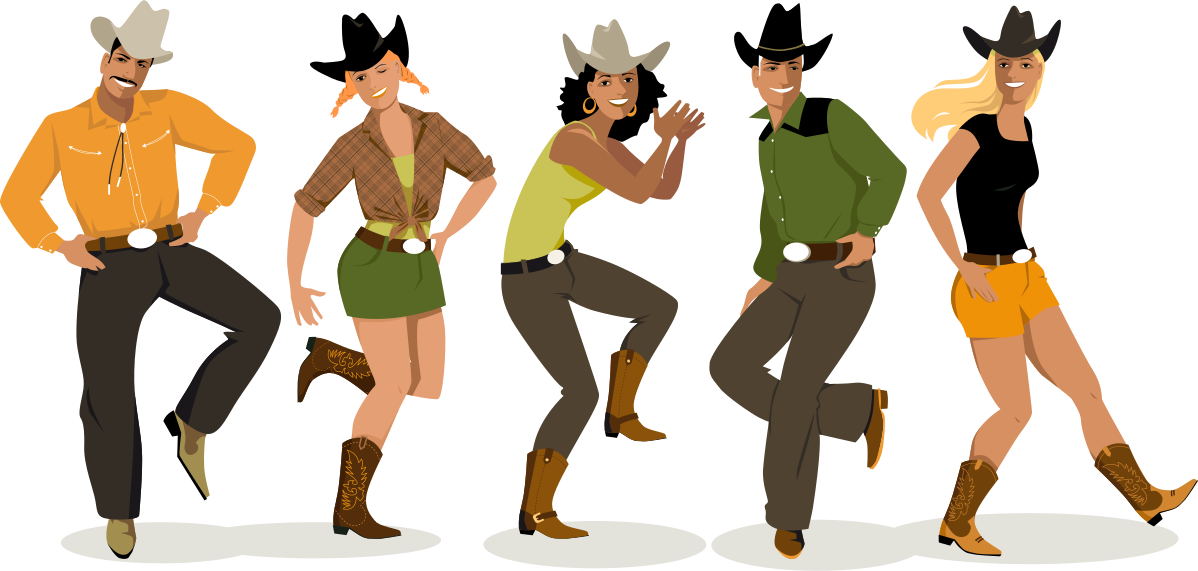
\includegraphics[width=140mm]{images/groupe.pdf}}
\put(15,-270){
\includegraphics[width=170mm]{images/groupededanseenligne-ombre.png}}
%\put(-3,-274){\href{https://alevisdanse.github.io}{\includegraphics[width=40mm]{images/qr-code.pdf}}}
%\put(-3,-274){\includegraphics[width=100mm]{images/Exposants.png}}
\put(20,-274){\includegraphics[width=80mm]{images/Vero'sBoutik.png}}
\put(90,-210){\includegraphics[width=100mm]{images/Charlie-Gon.png}}
\put(145,-30){\href{https://alevisdanse.github.io}{
\includegraphics[height=40mm]{logo/aldc-4couleurs-6.png}}}
\put(-5,-35){\href{https://country-rn10-13.webself.net/}{\includegraphics[height=50mm]{images/LOGO RN10 officiel-fi36141364x430.png}}}
\end{picture}


%%%%%%%%%%%%%%%%% DATE

\begin{center}
\fontsize{32pt}{36pt}\selectfont
Samedi \\
13 Décembre 2025\\
\fontsize{20pt}{24pt}\selectfont
  de 14h à 23h
\end{center}



\vspace*{25mm}



%%%%%%%%%%%%%%%%%%%%% BAL COUNTRY
\begin{center}
\fontspec{QTOKCorral-Ext}
\fontsize{100pt}{96pt}\selectfont
\begin{tikzpicture}
\node (a) at (0,0){};
\node (b) at (16,0){};
\node (aa) at (0.15,-0.15){};
\node (bb) at (16.15,-0.15){};
\draw[draw=none, postaction={decorate,decoration={text along path,text align=center,text color=yellow!20,text={BAL COUNTRY}}}] (aa) to [bend right=-20]  (bb);
\draw[draw=none, postaction={decorate,decoration={text along path,text align=center,text={BAL COUNTRY}}}] (a) to [bend right=-20]  (b);
\end{tikzpicture}
\end{center}


\vspace*{-20mm}


%%%%%%%%%%%%%%%%%%%%% Workshop
\begin{flushleft}
  % \begin{center}
  %\fontsize{32pt}{40pt}\selectfont

\fontsize{54pt}{54pt}
\fontspec{QTOKCorral-Ext}
\selectfont
~ Workshops Chrystel Arréou

~ Concert à 20h % Charlie Gon
%\end{center}
\end{flushleft}

%%%%%%%%%%%%%%%%%%%%% Animé par ...
% \begin{center}
%   \fontsize{32pt}{40pt}\selectfont

%   Animé par \\
% \fontsize{48pt}{48pt}
% \fontspec{QTOKCorral-Ext}
% \selectfont
% Chrystel Arréou et Carolyn Gaudin
% \end{center}

%%%%%%%%%%%%%%%%%%%%%

\vspace*{15mm}

\fontsize{20pt}{20pt}\selectfont
%Venez vous divertir dans une ambiance chaleureuse et conviviale

Salle Polyvalente de \\
Lévis-Saint-Nom\\
{\fontsize{14pt}{16pt}\selectfont
(78320, 6 Route d'Yvette)}

\vspace*{5mm}

Renseignements et \\
réservation obligatoire: \\
\href{mailto:alevisdanse@gmail.com?subject=Bal 13 decembre}{\texttt{\color{blue!50!black}alevisdanse@gmail.com}} \\
ou\\
\href{mailto:countryrn10@free.fr?subject=Bal 13 decembre}{\texttt{\color{blue!50!black}countryrn10@free.fr}}

\vspace*{5mm}

Entrée: \\
10 euros

\vspace*{-30mm}
\vfill

~\hfill\begin{minipage}{0.35\linewidth}
  \begin{center}
    Ouverture des portes
    à 13h15\\
    ~\\
    Restauration
    sur place\\
    ~\\
    Exposants
\end{center}
\end{minipage}

% {\fontsize{14pt}{16pt}\selectfont
% Nous sommes aussi sur FB: \raisebox{-8.5mm}{\includegraphics[width=20mm]{images/fb-aldc-qr-code.jpg}}}

\end{document}

\newpage

\begin{center}
Programme
\end{center}

\begin{description}
\item[13h30] Ouverture des portes
\item[14h] Ouverture du bal playlist CD
\item[15h] Workshop par Chrystel Arréou niveau débutant
\item[16h] Reprise de la playlist
\item[17h] Workshop par Chrystel Arréou niveau novice
\item[18h] Reprise de la playlist
\item[18h30] Apéro offert, pause restauration
\item[20h] Concert Charlie Gon
\item[22h] Reprise de la playlist
\end{description}

\vfill

\begin{center}
Bulletin d'inscription
\end{center}

à envoyer à alevisdanse@gmail.com

Nom, prénom

Club

reservation du repas (boisson + sandwich)

\begin{itemize}
\item sandwich jambon beurre cornichon
\item sandwich fromage
\end{itemize}

\end{document}
